\documentclass[a4paper]{article}

\usepackage{hyperref}

% Set up page size
\usepackage[margin=1.5cm, includefoot, footskip=30pt]{geometry}

% Nice way to display code
\usepackage{minted}

% Import images
\usepackage{graphicx}
\usepackage{amsmath}
\usepackage{multicol}

\usepackage{tikz}
\usetikzlibrary{calc}

\title{Modelling the effect of vaccinations using differential equations}
\author{Vince Knight}
\date{}


\begin{document}
\maketitle


\section{Introduction}\label{sec:introduction}


The World Health Organisation estimates that the measles vaccination has saved
more than 17 million lives since 2000~\cite{who}.  It is possible to model the
effect of vaccination using differential equations. The model considered here is
called an SIR model which is a compartementalised model of infection where
individuals can be in one of 3 states:

\begin{itemize}
    \item Susceptible (S): members of the population who may become infected;
    \item Infected (I): infected members of the population who will eventually
        recover;
    \item Recovered (R): recovered members of the population, not that
        mathematically death is here equivalent to recovery.
\end{itemize}

Figure~\ref{fig:sir_model} shows this diagrammatically.

\begin{figure}[!hbtp]
    \begin{center}
        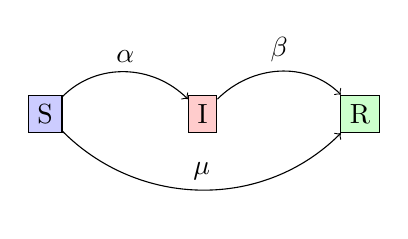
\begin{tikzpicture}
            \node [draw, fill=blue!20] (S) at (0, 0) {S};
            \node [draw, fill=red!20] (I) at ($(S) + (2, 0)$) {I};
            \node [draw, fill=green!20] (R) at ($(I) + (2, 0)$) {R};

            \draw [->] (S) edge [out=45, in=135] node [above] {\(\alpha\)} (I);
            \draw [->] (I) edge [out=45, in=135] node [above] {\(\beta\)} (R);
            \draw [->] (S) edge [out=-45, in=-135] node [above] {\(\mu\)} (R);
        \end{tikzpicture}
    \end{center}
    \caption{The SIR model}
    \label{fig:sir_model}
\end{figure}

The parameters of the model shown in Figure~\ref{fig:sir_model} are:

\begin{itemize}
    \item \(\alpha\) the infection rate;
    \item \(\beta\) the recovery rate;
    \item \(\mu\) the vaccination percentage;
\end{itemize}

This can be expressed mathematically:

\begin{align}
    \frac{dS}{dt} &= - \alpha I S - \mu S\\
    \frac{dI}{dt} &=  \alpha I S - \beta I\\
    \frac{dR}{dt} &=  \mu S + \beta I
\end{align}

In the next section we will use Sympy to attempt to solve these equations
analytically:

\section{(Not) finding an exact solution}

It is possible to use Sympy to solve systems of differential equations, however
when attempting to do this here it appears to fail:

\begin{minted}{python}
>>> import sympy as sym
>>> S, I, R = sym.Function("S"), sym.Function("I"), sym.Function("V")
>>> N, mu, alpha, beta, t = sym.symbols("N, mu, alpha, beta, t")
>>> eq1 = sym.Derivative(S(t), t) - (- alpha * S(t) * I(t) - mu * R(t))
>>> eq2 = sym.Derivative(I(t), t) - (alpha * I(t) * S(t) / N  - beta * I(t))
>>> eq3 = sym.Derivative(R(t), t) - (beta * I(t) + mu * R(t))
>>> sym.dsolve((eq1, eq2, eq3))
NotImplementedError                       Traceback (most recent call last)
...
\end{minted}

I believe that this is due to the complexity of the differential equations that
Sympy is unable to handle analytically. An exact solution of the model without
vaccination is obtained in~\cite{harko2014exact}.
In the next section we will however solve these equations numerically.

\section{Solving the equations numerically and the effect of vaccination rates}

We can use a numerical integration technique to solve these equations
numerically. The technical publication describing the specific algorithm used is
described in~\cite{radhakrishnan1993description}.

First we create a function that gives expressions for the
derivatives at any given point in time:

\begin{minted}{python}
>>> def dx(x, t, alpha, beta, mu):
...     return (- alpha * x[1] * x[0] - mu * x[0],
...             alpha * x[1] * x[0]  - beta * x[1],
...             beta * x[1] + mu * x[0])
\end{minted}

We can then plot a number of different scenarios as shown in
Figure~\ref{fig:scenarios}. Here is the code that corresponds to the first plot:

\begin{minted}{python}
>>> alpha = 1 / 1000  # Every 1000 interactions leads to infection
>>> beta = 1 / 5  # take 5 time units to recover
>>> N = 10 ** 4  # Population of 10 thousand people
>>> mu = 0  # 0 vaccination rate
>>> ts = np.linspace(0, 10, 5000)
>>> xs = integrate.odeint(func=dx, y0=np.array([N - 1, 1, 0]), t=ts, args=(alpha, beta, mu))
>>> S, I, R = xs.T
>>> plt.figure()
>>> plt.plot(ts, S, label="Susceptibles")
>>> plt.plot(ts, I, label="Infected")
>>> plt.plot(ts, R, label="Recovered")
>>> plt.legend()
>>> plt.title(f"$\max(I)={round(max(I))}$ ($\\alpha={alpha}$, $\\beta={beta}$,
$\mu={mu}$)");
\end{minted}

\begin{figure}[!hbtp]
    \begin{center}
        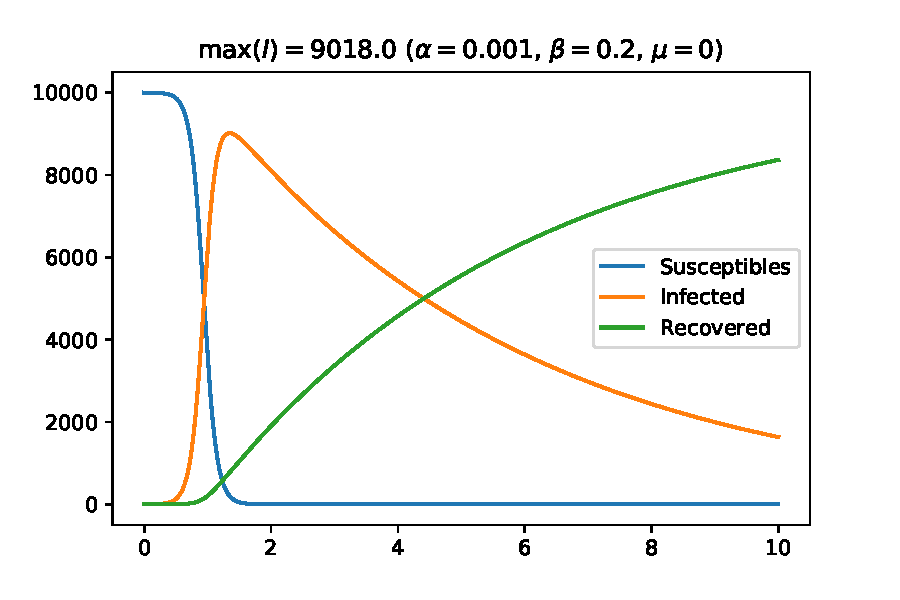
\includegraphics[width=.3\textwidth]{base_scenario.pdf}
        ~
        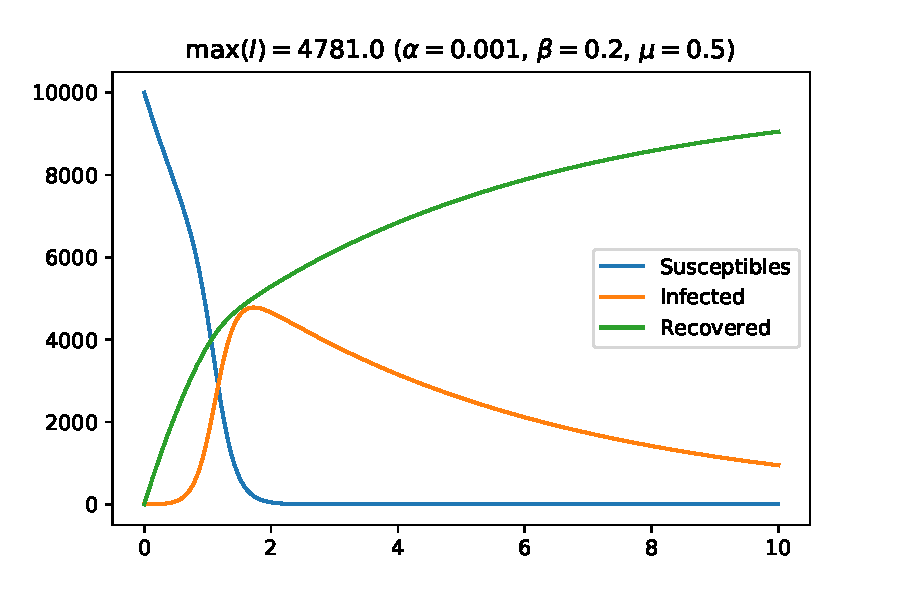
\includegraphics[width=.3\textwidth]{moderate_vaccination_rate.pdf}
        ~
        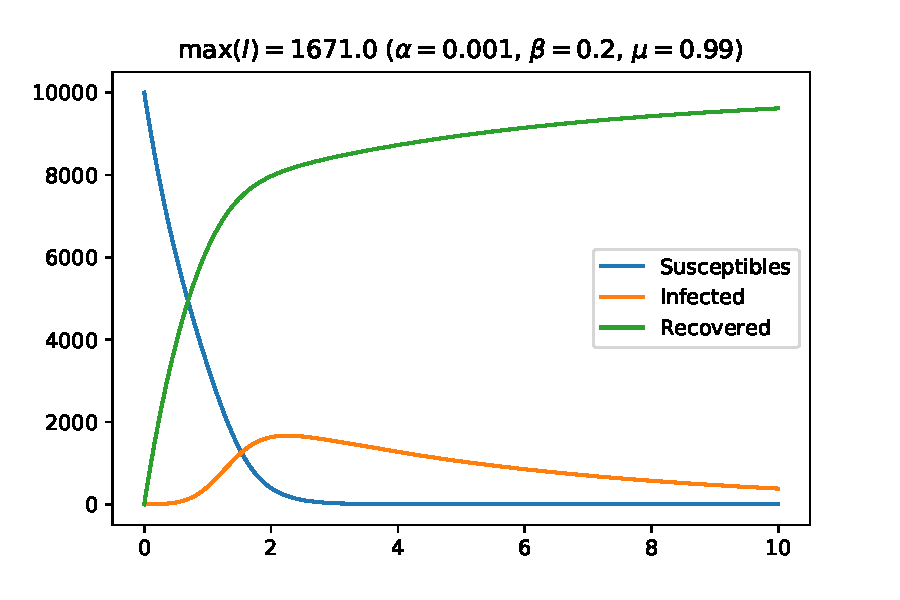
\includegraphics[width=.3\textwidth]{high_vaccination_rate.pdf}
        \caption{The evolution of the population for different vaccination rates}
        \label{fig:scenarios}
    \end{center}
\end{figure}

It is also possible to compute the maximum percentage of infection as a function
of the vaccination rate:

\begin{minted}{python}
>>> vaccination_rates = np.linspace(0, 1, 500)
>>> max_percent_of_infected = []
>>> for mu in vaccination_rates:
...     xs = integrate.odeint(func=dx, y0=np.array([N - 1, 1, 0]), t=ts, args=(alpha, beta, mu))
>>> S, I, R = xs.T
>>> max_percent_of_infected.append(max(I) / N)
>>> plt.figure()
>>> plt.plot(vaccination_rates, max_percent_of_infected)
>>> plt.xlabel("Vaccination rate")
>>> plt.ylabel("% of population infected");
\end{minted}

This is shown in Figure~\ref{fig:effect_of_vaccination_rate}.

\begin{figure}[!hbtp]
    \begin{center}
        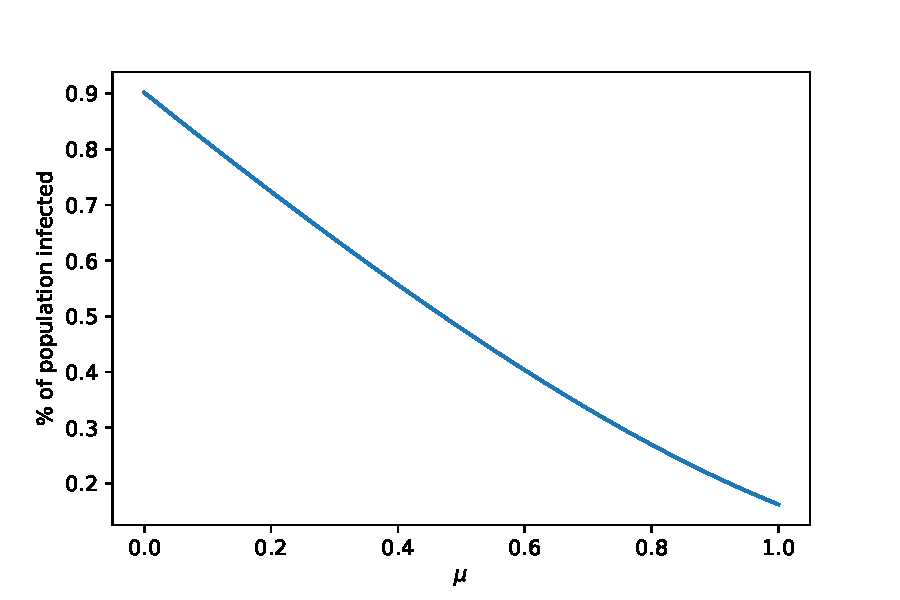
\includegraphics[width=.6\textwidth]{effect_of_vaccination_rate.pdf}
        \caption{The effect of vaccination rate on maximum infection percentage}
        \label{fig:effect_of_vaccination_rate}
    \end{center}
\end{figure}

\section{Conclusion}

We see in our model that a large vaccination rate is required to ensure a high
level of immunity (ie a low maximum level of total infection). This type of
approach uses differential equations to model the interactions of individuals
and the spread of disease, finally we solve these equations using techniques
from numerical analysis.

\bibliographystyle{plain}
\bibliography{bibliography.bib}


\end{document}
